%
% $RCSfile: composite.tex,v $
%
% Copyright (C) 2002-2008. Christian Heller.
%
% Permission is granted to copy, distribute and/or modify this document
% under the terms of the GNU Free Documentation License, Version 1.1 or
% any later version published by the Free Software Foundation; with no
% Invariant Sections, with no Front-Cover Texts and with no Back-Cover
% Texts. A copy of the license is included in the section entitled
% "GNU Free Documentation License".
%
% http://www.cybop.net
% - Cybernetics Oriented Programming -
%
% http://www.resmedicinae.org
% - Information in Medicine -
%
% Version: $Revision: 1.1 $ $Date: 2008-08-19 20:41:06 $ $Author: christian $
% Authors: Christian Heller <christian.heller@tuxtax.de>
%

\subsubsection{Composite}
\label{composite_heading}
\index{Composite Pattern}
\index{Directed Acyclical Graph}
\index{DAG}
\index{Tree}
\index{Whole-Part Pattern}
\index{Recursion}

A hierarchical object structure, also called \emph{Directed Acyclical Graph}
(DAG) or \emph{Tree}, can be represented by a combination of classes called
\emph{Composite} pattern \cite{gamma1995}. It describes a \emph{Component} that
may consist of \emph{Children} (figure \ref{composite_figure}), which makes it
comparable to the \emph{Whole-Part} pattern. The difference is that the
\emph{Composite} is a more generalised version, with a dynamically extensible
number of child (part) objects. The \emph{Composite} is a pattern based on
\emph{Recursion}, which is one of the most commonly used programming techniques
at all. The pattern's split into \emph{Leaf-} and \emph{Composite} sub classes
helps distinguish primitive- from container objects. A composite tree node
holds objects of type \emph{Component}.

\begin{figure}[ht]
    \begin{center}
        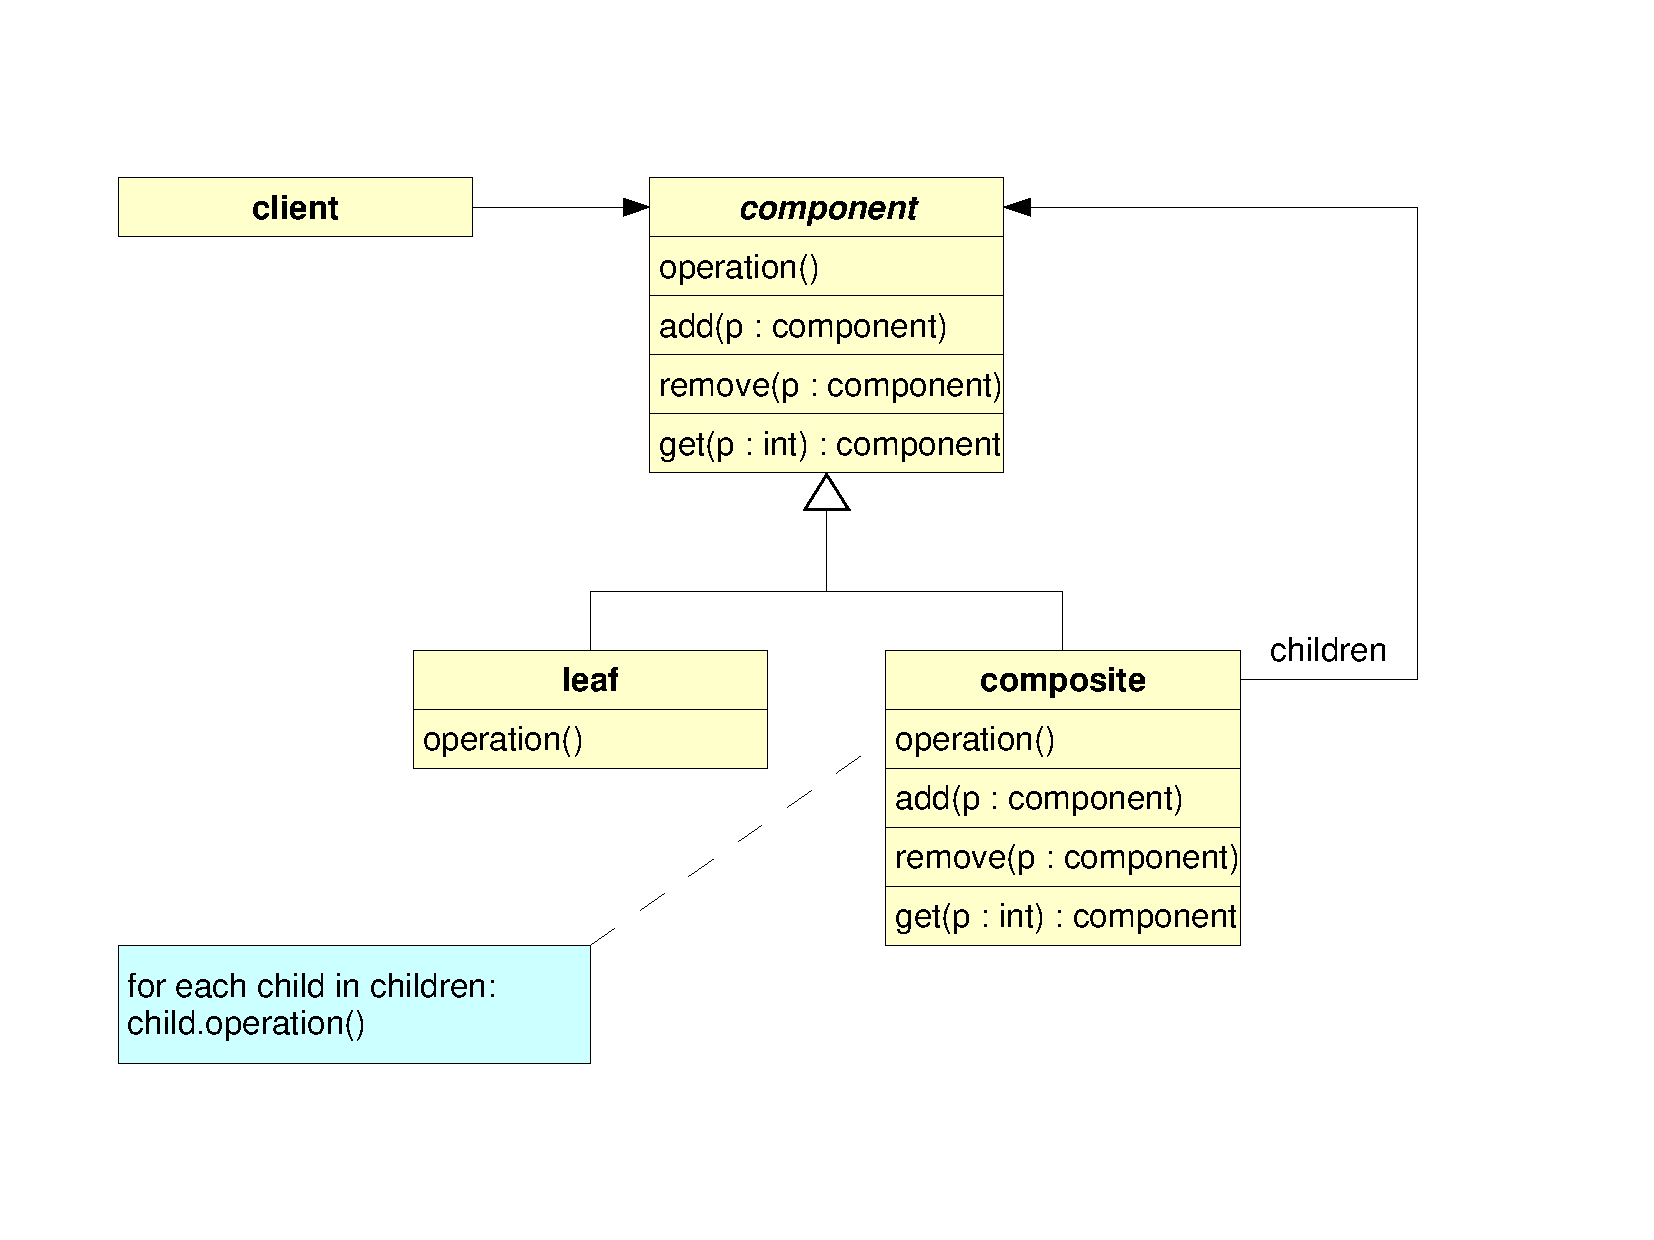
\includegraphics[scale=0.3,angle=-90]{graphic/composite.pdf}
        \caption{Composite Pattern}
        \label{composite_figure}
    \end{center}
\end{figure}

The knowledge schema introduced in chapter \ref{knowledge_schema_heading} has
container capabilities, like the composite pattern. It does, however, not
distinguish between composite and leaf nodes, and not use inheritance.
